\documentclass[11pt,a4paper]{article}
\usepackage{fontspec}
\setmainfont{Times New Roman}
\setmonofont{Consolas}
\usepackage[margin=2.3cm]{geometry}
\usepackage{amsmath,amssymb,graphicx,booktabs,tabularx,array}
\usepackage{enumitem,caption,xurl}
\usepackage[unicode,hidelinks]{hyperref}
\setlength{\emergencystretch}{2em}
\setlength{\parskip}{3pt}
\setlist{itemsep=2pt,topsep=3pt,leftmargin=*}
\newcommand{\code}[1]{\texttt{\detokenize{#1}}}
\newcolumntype{Y}{>{\raggedright\arraybackslash}X}
\title{\textbf{Link-Quality Forecast Accuracy Does Not Translate
into Routing Gains in UAV Relay Networks}}
\author{Nguyen Dinh Tam\thanks{Corresponding author: \href{mailto:23521389@gm.uit.edu.vn}{23521389@gm.uit.edu.vn}.} \and Vo Cong Vinh}
\date{University of Information Technology, VNU-HCM\\November 2026}
\begin{document}
\maketitle
\begin{abstract}
Learned link-quality forecasting for UAV routing is a well-populated research
direction, but most models are evaluated by forecast accuracy rather than by
the network service they deliver. This paper tests that gap directly: does a
learned forecaster improve service once it is placed inside the control loop
and compared against a tuned baseline? A graph neural network (GNN) regresses
the mean probe reception ratio over the next five seconds from positions,
velocities and causal link measurements. The same weight-locked forecaster then
drives two different actions inside ns-3.45: data route selection and relay
repositioning. Three studies were pre-registered before any new simulation was
run; the first two comprise 80 validation and 192 test episodes on fresh audited seeds,
over chains of five or seven UAVs, with arms compared pairwise within seed
blocks. Locked results: for routing, the graph forecast raises the packet
delivery ratio (PDR) by 0.66 percentage points over current measured quality,
95\% confidence interval [0.38, 1.00]; for placement control, forecasting saves
only 0.20 disconnected seconds relative to a reactive trigger, confidence
interval [$-1.05$, $1.45$], so the primary endpoint was not met. Three
exploratory analyses on fresh seeds explain both outcomes and form the main
contribution. First, the ranking by forecast error runs \emph{opposite} to the
ranking by service: an EWMA filter with coefficient 0.1 has the worst mean
squared error of the three estimators yet the highest PDR, beating the GNN by
0.31 percentage points [0.04, 0.61]. Second, the entire GNN gain is reproduced
by that one-parameter filter once its coefficient is tuned, so the benefit
attaches to a more stable quality estimate rather than to the value of forecast
information. Third, a geometric bound shows that ideally equispaced relays
still leave 26.09 disconnected seconds per episode, so the reactive trigger
already attains roughly 94\% of the achievable reduction and almost no
headroom remains for forecasting. A third study, pre-registered and run on
fresh seeds, then tests the most important of those three conclusions: when both
quality sources are given the same smoothing parameter and each coefficient is
selected on a separate tuning set, the PDR difference between the GNN forecast
and the smoothed measurement is 0.08 percentage points, confidence interval
[$-0.11$, $0.29$], with no difference detected. The practical conclusion is that in this
scenario family a cheaper stable estimator beats a learned forecaster, and
forecast accuracy is not a substitute for a closed-loop service experiment.
Limitations include centralized telemetry that does not yet contend for the
channel, a single training seed, a single chain topology family and no flight
trial.
\end{abstract}
\noindent\textbf{Keywords:} UAV networks; graph neural networks; link quality;
routing; closed-loop evaluation; pre-registration.
\section{Introduction}
In a chain of relaying UAVs, link degradation can cause packet loss or
disconnect the source from the destination. Link forecasting can support two
distinct decisions: which path packets take, and where relays are placed. Many
works already use forecasting, position information or GNNs for UAV routing, so
the contribution to be examined here is not a claim of first use of those
mechanisms. The issue is how they are evaluated: a better forecasting model
does not by itself demonstrate a better controller, and most link-quality
estimators are assessed offline by accuracy~\cite{cerar}.

The paper therefore asks its questions at the service level. First, does the
GNN forecast improve the packet delivery ratio (PDR) over current measured
quality when the route-selection rule is held fixed? Second, does it reduce
disconnected seconds when routing and the relay placement rule are held fixed
and only the motion trigger changes? Third, and most importantly, if a gain
exists, how much of it survives once the simple baseline is tuned, and does it
track forecast accuracy? The three consecutive studies are labelled v8, v9 and
v10 to link them to the experiment records in the code repository: v8 and v9
test the two actions, and v10 is a confirmatory study pre-registered after their
results were seen.

The contributions are fourfold:
\begin{itemize}
\item A design that routes \emph{one weight-locked forecaster} into two
different actions inside the same simulator, with the same binary, the same
action rules and the same seed blocks, so that observed differences are
attributable to the quality source rather than to system configuration.
\item Quantitative evidence that the ranking by forecast error runs opposite to
the ranking by service on the same traces: the estimator with the worst error
yields the highest PDR (Section~\ref{sec:posthoc}).
\item An ablation separating \emph{smoothing} from \emph{forecasting}: the whole
GNN gain is reproduced by a tuned one-parameter EWMA filter. This conclusion is
then checked by a pre-registered confirmatory study in which both quality
sources are tuned on a separate tuning set (Section~\ref{sec:v10}).
\item A geometric bound for the relay placement problem showing that the
reactive rule already attains about 94\% of the achievable reduction in
disconnection, so the negative result on the placement branch has a
quantitative explanation rather than merely reflecting low statistical power.
\end{itemize}
The whole procedure was pre-registered~\cite{nosek}: endpoints, test order and
stopping rules were written down before the first cell was run, and unfavourable
results are reported.
\section{Related work}
\subsection{Link-quality-aware routing}
FANETs are characterised by high mobility and rapidly changing
topology~\cite{bekmezci}, and both the general UAV network
surveys~\cite{gupta,hayat} and the routing-specific
surveys~\cite{arafat,lakew} treat link durability as a decisive factor.
OLSR~\cite{rfc3626} selects routes by hop count: a link counts as usable as
soon as HELLO messages traverse it in both directions, and its packet loss does
not enter the path cost. OLSRv2~\cite{rfc7181} adds a link-metric framework, but
the OLSR implementation in ns-3 follows RFC 3626. ETX~\cite{decouto} and
ETT~\cite{draves} replace hop count with a cost reflecting loss and bandwidth;
olsrd~\cite{olsrd} brings ETX into OLSR and is the natural distributed baseline
for any link-quality-aware routing method.

\subsection{Link-quality forecasting and GNNs}
Link-quality estimation is a research direction in its own right, ranging from
packet-statistics estimators~\cite{baccour} to machine-learning
models~\cite{cerar}. GNNs learn node representations through iterated message
passing: GCN~\cite{kipf}, GraphSAGE~\cite{graphsage} with neighbour aggregation
that generalises to graphs unseen during training, and GAT~\cite{gat} with
attention weights per neighbour. A UAV network is naturally a time-varying
graph, which makes GNNs a reasonable candidate. In wired networks,
RouteNet~\cite{routenet} uses a GNN to predict delay and loss from topology and
routing. In UAV networks, Bai et al.~\cite{bai2025} predict links with a dynamic
GNN and take GraphSAGE and node2vec themselves as baselines;
GNNPPOR~\cite{gnnppor} couples a GNN with PPO for path selection in FANETs; and
a recent review~\cite{drones2026} surveys GNN applications across UAV systems.
Within FANETs, QMR~\cite{qmr} uses Q-learning for multi-objective next-hop
selection, and XGBoost~\cite{xgboost} is the strong tabular baseline that any
GNN evaluation needs. Predictive-OLSR~\cite{rosati2013} uses GPS and relative
velocity to adjust ETX weights, while OLSR-LCN~\cite{liu2025} combines link
lifetime, interference and node load. In other words, \emph{using forecasting,
position information or GNNs for UAV routing is no longer a new idea}; the open
question is what such a model is actually worth when measured by service.

\subsection{The gap between accuracy and service benefit}
Cerar et al.~\cite{cerar} observe in their survey that most link-quality
estimation models are evaluated offline by accuracy and are rarely placed
inside a routing loop to measure the service benefit. Shi et al.~\cite{shi2024}
show that several families of machine-learning models converge on the same
accuracy ceiling imposed by channel stochasticity. In other fields this gap is
well documented: in autonomous driving, the ranking of motion predictors shifts
substantially when evaluation moves from open loop to closed
loop~\cite{closedloop2025}; in information retrieval, much of the reported gain
of neural models disappears once baselines are properly tuned~\cite{lin2018};
and in machine learning for partial differential equations, 79\% of surveyed
articles compare against a weak baseline~\cite{mcgreivy2024}.
Pre-registration~\cite{nosek} is a direct countermeasure against reselecting a
configuration after seeing the results.

\subsection{Relay placement}
Work on relay trajectory optimisation~\cite{zeng2016} controls UAV positions to
maximise throughput, usually with an analytic channel model and the assumption
that traffic follows the relay chain the controller selects. Software-defined
UAV networks~\cite{abir} employ a controller with a global view; the drawbacks
usually cited are signalling overhead, control delay and scalability. This work
does not solve the optimal trajectory problem; it keeps a fixed equispacing
placement rule in order to isolate the \emph{trigger timing}, and additionally
measures a geometric bound so that the distance between that rule and the best
achievable outcome is known.

\subsection{The targeted gap}
To the best of our knowledge, no prior work in UAV networking (i) drives two
different actions from one weight-locked forecaster inside the same simulator,
(ii) pre-registers the endpoints and the test order and then reports
unfavourable results as well, and (iii) contrasts the ranking by forecast error
with the ranking by service on the same set of traces. Those are the three
points this paper targets.

\section{Materials and methods}
Figure~\ref{fig:design} summarises the two comparisons.
\begin{figure}[htbp]
\centering
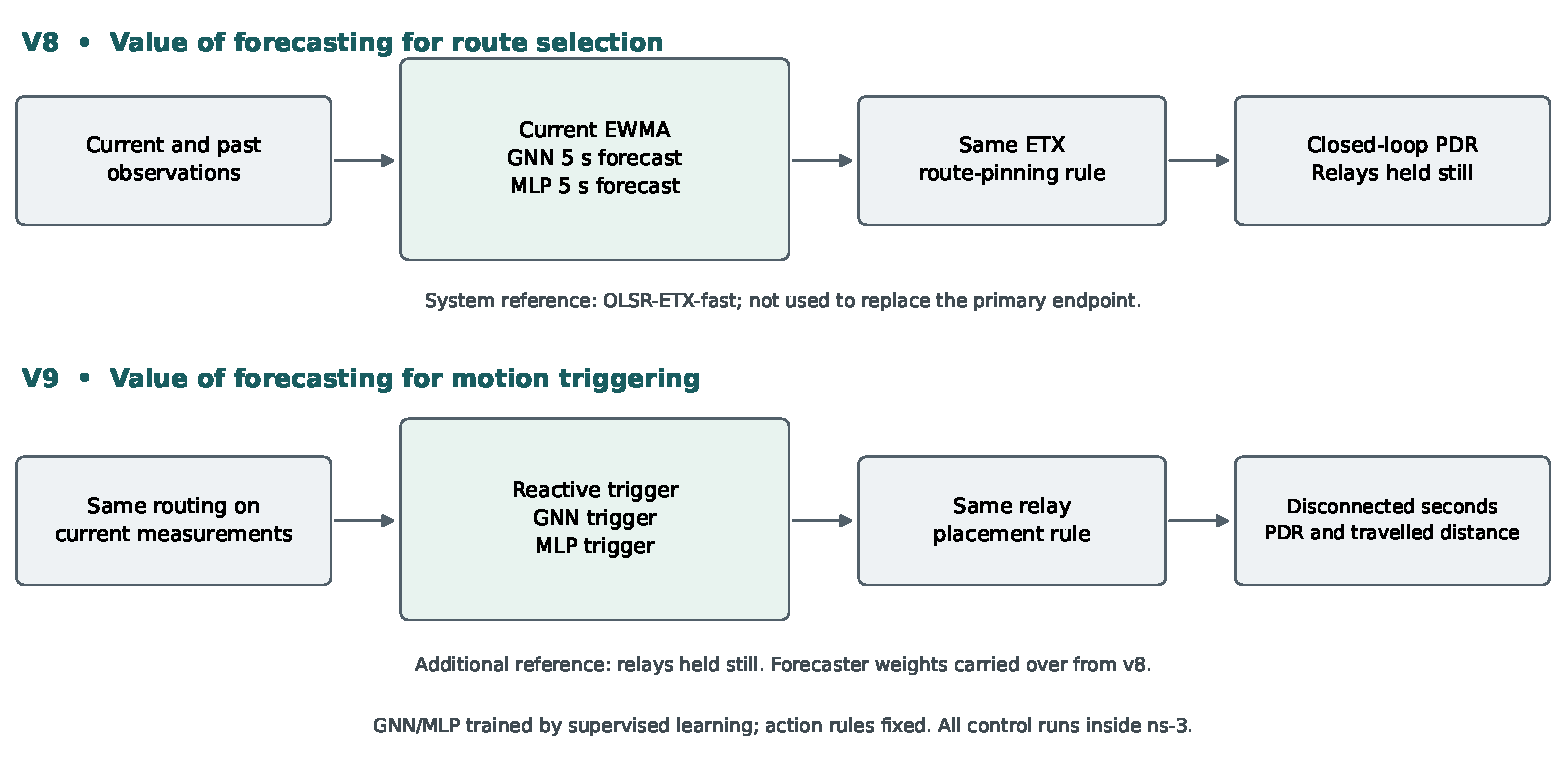
\includegraphics[width=\linewidth]{images/fig_v8_v9_design.pdf}
\caption{Separating forecasting for route selection from forecasting for motion triggering.}\label{fig:design}
\end{figure}
\subsection{Problem statement}
At time $t$ the network is a graph $G_t=(V,E_t)$ whose vertices $V$ are the
UAVs. Each edge $e=(a,b)$ carries a measured quality $d_e(t)\in[0,1]$, the probe
reception ratio within a one-second window. A quality estimator produces the
decision variable $x_e(t)$ in one of two families:
\begin{align}
\text{measure and smooth:}\quad & x_e(t)=\alpha\, d_e(t)+(1-\alpha)\,x_e(t-1),\label{eq:ewma}\\
\text{learned forecast:}\quad & x_e(t)=\hat g_e(t)\approx
\frac{1}{H}\sum_{\tau=t+1}^{t+H} d_e(\tau),\qquad H=5\ \text{s}.\label{eq:fore}
\end{align}
Equation~\eqref{eq:ewma} is a one-parameter EWMA; $\alpha=0.5$ is the
configuration inherited from earlier studies and serves as the v8 baseline.
Equation~\eqref{eq:fore} is the GNN regressor, trained by supervised learning on
historical data and using only causal observations up to time $t$.

Both actions consume the same $x$. The routing action selects the path
\begin{equation}
\pi_t=\arg\min_{P\in\mathcal{P}(s,d)}\ \sum_{e\in P}\frac{1}{\max(x_e(t),\varepsilon)},
\label{eq:etx}
\end{equation}
that is, an ETX-style cost~\cite{decouto} evaluated on $x$ rather than on raw
measurements, under the route-pinning rule with margin and dwell described in
Section~\ref{sub:v8}. The placement action uses the best bottleneck path quality
\begin{equation}
Q(t)=\max_{P\in\mathcal{P}(s,d)}\ \min_{e\in P} x_e(t),
\label{eq:bottleneck}
\end{equation}
and triggers a fixed relay motion rule when $Q(t)$ falls below a threshold.

The central distinction of this paper lies between two measures taken on the
same $x$. \emph{Forecast} quality is measured by the mean squared error
$\mathrm{MSE}=\mathbb{E}\big[(x_e(t)-\frac{1}{H}\sum_\tau d_e(\tau))^2\big]$,
computed offline over traces. \emph{Service} quality is measured by PDR and
disconnected seconds, computed in closed loop while $x$ actually
drives~\eqref{eq:etx} or~\eqref{eq:bottleneck}. The question of the paper is
whether these two measures rank estimators in the same order.

\subsection{Environment and experimental design}
The experiments use ns-3.45~\cite{ns3}, Wi-Fi 802.11g and OLSR~\cite{rfc3626} on
chains of five or seven UAVs. Source and destination sit at the two ends of the
chain and the remaining nodes act as relays. Each episode lasts 240~s with a
256~kbps UDP main flow and two 128~kbps background flows. Two contexts are used,
static and gradual: the endpoints either stay still or separate from second 30.
The binary and runtime are inherited from the previous studies, including the
OLSR-ETX baseline implemented by the group and an ARP DeadTimeout of 1~s. Every
arm uses the same binary, channel, traffic and block seeds.

The simulation area is $1800\times1200$~m with altitudes of 50--150~m. The
initial spacing between consecutive nodes is nominally 24~m with up to 0.72~m of
jitter per coordinate. The channel combines log-distance path loss (exponent
2.2, 40~dB reference loss at 1~m) with Nakagami fading ($m=3$, $1.5$ and $1$ for
distances below 96~m, 96--180~m and above 180~m respectively). Transmit power is
20~dBm and the PHY rate is fixed at 6~Mbps. The nominal 240~m range is used to
set receiver sensitivity and is not a distance-based link cut-off. Warmup lasts
10~s; probes are broadcast every 0.05~s and aggregated over a one-second window;
the main flow uses 512~B packets, 15{,}000 packets per episode.

The protocol was written before the new simulations. Each phase packages the
source code, model, seed plan and runtime identity under SHA-256; the test phase
inherits exactly the sources and model of validation. Each cell runs once, and a
four-worker queue holds a server-wide lock. Validation comprises 80 cells (two
static and eight gradual per configuration, four arms); the test comprises 192
cells (four static and 20 gradual per configuration, four arms). No model was
reselected on the basis of validation or test service results.

\subsection{Link forecasting and the control model}
The model forecasts the mean probe reception ratio over the next five seconds,
not a link survival probability. The development data consist of 48 HOLD traces
from the v7 test phase for fitting and 20 HOLD validation traces from v7 for
epoch selection. These already-observed data are treated wholly as development
data for the new studies; v8 and v9 use independent audited seeds. Each episode
yields 236 valid forecast origins, giving 11{,}328 fitting samples and 4{,}720
epoch-selection samples; correlated frames are not treated as independent
replicates when testing control effectiveness.

The inputs comprise only current and past observations. The eight node features
are coordinates relative to the formation centroid, velocity, neighbour degree
and mean reception ratio. The seven edge features are distance, RSSI, current
reception ratio, an EWMA with coefficient 0.5, the reception-ratio difference,
the separation velocity and the magnitude of relative velocity. Coordinates and
distances are divided by 240~m, velocities by 10~m/s, and RSSI is transformed as
$(\mathrm{RSSI}+90)/40$ with missing values encoded as $-100$~dBm. An edge
participates in message passing only if its current reception ratio is at least
0.1. No future mission trajectory is read.

Edge-SAGE comprises two mean-aggregation layers with edge features, 64
dimensions and ReLU, followed by a 64-dimensional node-pair decoder with a
sigmoid and symmetrised logits. The GNN has 19{,}137 parameters. The MLP drops
the two learned message-passing branches, leaving 13{,}505 parameters, and still
retains the node-degree feature. The ablation therefore does not separate the
effect of message passing from the difference in model capacity. Both use MSE
loss, Adam with learning rate 0.001, weight decay $10^{-5}$, batch size 128,
gradient clipping at norm 5, at most 60 epochs, patience 10 and seed 20261123.
The GNN and MLP selected epochs 58 and 59. The largest discrepancy between the
NumPy and PyTorch inference paths over 40 check snapshots is
$1.19\times10^{-7}$. This is supervised learning; neither study uses
reinforcement learning.

\subsection{Routing study v8}\label{sub:v8}
The four arms are current quality (\code{lq-route}), the GNN forecast
(\code{gnn-route}), the MLP forecast (\code{mlp-route}) and OLSR-ETX-fast. The
three route-pinning arms share the same ETX rule with margin 1.0, a three-step
warmup and a five-second dwell; the broken-link check still uses a current
reception ratio below 0.1. ETX-fast uses the HELLO interval of 0.5~s and TC
interval of 1.25~s selected in v7. Relays stay still, and each gradual endpoint
has a nominal speed of 1~m/s multiplied by a factor in $[0.85, 1.15]$ drawn per
layout seed. The source moves along $+y$ and the destination along $-y$; the
same seed yields the same endpoint motion across arms. Validation checks
technical criteria only: cell count, route correctness, simulator flags,
forecasting, counters and background flows, no startup blackout and no relay
motion. The go decision does not depend on any PDR difference.

The three tests in fixed order are the PDR difference of GNN minus current, GNN
minus MLP, and then GNN minus ETX-fast. A step succeeds when the lower bound of
the 95\% confidence interval is positive; an affirmative interpretation is
permitted only when every preceding step has succeeded. Test MSE is measured
separately for the GNN, the MLP and the EWMA on the same \code{lq-route} traces,
kept apart from closed-loop PDR.

\subsection{Placement study v9}
Study v9 keeps the v8 weights unchanged and routes on current quality in every
arm. The arms are stationary relays, reactive motion triggering, GNN triggering
and MLP triggering. The best path quality is $Q=\max_P\min_{e\in P}q_e$. After
three frames, the reactive arm triggers if the current EWMA has $Q<0.70$ in two
consecutive frames; the GNN and MLP arms add the analogous condition on the
forecast. A forecast edge is used only if its current measurement is at least
0.1.

Relays are ordered by their projection onto the line joining the current
endpoints and then directed towards points that divide that segment equally. The
limits are 8~m/s, 400~m per relay, a 1~m deadband, at most ten steps per burst
and a five-step rest. Motion stops early after three frames in which the current
quality, and the forecast where applicable, are at least 0.80. An in-step
minimum separation check must reach 5~m; otherwise the relay motion command is
set to zero. This rule is identical in every arm with motion, only the trigger
differs.

The nominal speed of each gradual endpoint rises to 2~m/s, retaining the
per-seed random factor of v8, in order to create a disconnection challenge; this
differs from the 1~m/s fitting distribution. Validation requires the technical
and safety criteria to pass and at least 8 of 16 stationary gradual baseline
episodes to lose connectivity for at least five seconds. If that fails, the test
does not run and the speed is not retuned within the same study.

The primary endpoint is the disconnected seconds of the reactive arm minus those
of the GNN arm; the subsequent steps consider the PDR of GNN minus reactive, and
then the disconnected seconds of MLP minus GNN. Disconnection means that source
and destination lie in different connected components of the probe graph
thresholded at 0.5, counted over frames 1--240. The seconds during which OLSR
has no route, and PDR, are separate quantities. This is a measured
graph-threshold partition, not a proof that no radio packet whatsoever could
cross between components. Travelled distance, longest outage, number of motion
bursts and background-flow PDR are descriptive.

\subsection{Statistical analysis and cost}
Each comparison keeps all four arms within the same seed block; the bootstrap
draws 10{,}000 resamples over the 40 gradual test blocks, 20 per configuration,
balanced between n5 and n7, with RNG seed 20261120. The
bootstrap~\cite{efron1993} is applied at the scenario level so that correlations
between arms are preserved. Negative results and gated steps are still
reported. A confidence interval containing zero does not establish equivalence.
Static results are descriptive only, with eight blocks.

The collector measures whole-decision latency on an eight-vCPU KVM virtual
machine (Intel Xeon Silver 4110 at 2.10~GHz) running four workers, each with
compute libraries restricted to a single thread. Probes are emitted in every
arm; centralized telemetry and commands are not yet transmitted as
channel-contending packets. Computation time is not converted into end-to-end
control delay, bytes are not converted into airtime, and travelled distance is
not converted into energy.

Signalling overhead was measured in study v7 with the same binary and runtime,
so the following figures apply to the v8 configuration: about 0.29~kB/s for
plain OLSR, 0.44~kB/s for OLSR-ETX, 1.78~kB/s for OLSR-ETX with 0.5~s HELLO, and
about 5.55~kB/s for route pinning, comprising 0.29~kB/s of fallback OLSR,
5.02~kB/s of probes and an estimated 0.25~kB/s of reports to the controller.
These are IP-layer bytes plus the estimated reporting component and are not
converted into a percentage of channel capacity. Probes are emitted in every
arm, so probe airtime is common across arms, but it is charged only to the
methods that consume probes. The centralized reporting component does not
contend for the channel in simulation. Every comparison between route pinning
and OLSR-ETX in this paper must therefore be read as an upper bound for a
partially idealized centralized controller.

\section{Results}
\subsection{Forecasting for route selection}

Validation of v8 yielded 80/80 valid cells; the go decision passed and the test
yielded 192/192 valid cells.

Table~\ref{tab:v8primary} presents the comparisons in the pre-locked order.

\begin{table}[htbp]
\centering\small
\begin{tabularx}{\linewidth}{@{}Yp{1.8cm}p{3.4cm}p{1.7cm}@{}}
\toprule
\textbf{Comparison}&\textbf{Difference}&\textbf{95\% CI}&\textbf{Gate}\\\midrule
H1: \code{gnn-route} $-$ \code{lq-route}&0.66&[0.38, 1.00]&Met\\
H2: \code{gnn-route} $-$ \code{mlp-route}&0.38&[0.12, 0.67]&Met\\
H3: \code{gnn-route} $-$ \code{olsr-etx-fast}&5.75&[5.07, 6.45]&Met\\
\bottomrule
\end{tabularx}
\caption{Routing test: PDR in percentage points. Each comparison uses 40 fresh gradual blocks.}\label{tab:v8primary}
\end{table}


The primary endpoint was met and the subsequent steps follow the sequential gate
shown in the table. Route integrity was correct in 144/144 inspected episodes
and all technical checks passed.

H3 compares a centralized controller against a distributed protocol in a setting
where telemetry and commands are not transmitted as channel-contending packets.
The difference of 5.75 percentage points is therefore an upper bound for this
centralized configuration rather than the gain expected once signalling is fully
simulated; the corresponding signalling cost is 5.55~kB/s against 1.78~kB/s.

Table~\ref{tab:v8meanspaper} records the PDR, disconnected time and travelled
distance of each arm.

\begin{table}[htbp]
\centering\small
\begin{tabularx}{\linewidth}{@{}Yp{3.4cm}p{2.2cm}p{2.5cm}@{}}
\toprule
\textbf{Arm}&\textbf{PDR (\%, mean $\pm$ SD)}&\textbf{Disconnected (s)}&\textbf{Distance (m)}\\\midrule
\code{gnn-route}&96.01 $\pm$ 2.58&31.65&0.00\\
\code{lq-route}&95.35 $\pm$ 2.92&31.77&0.00\\
\code{mlp-route}&95.64 $\pm$ 2.68&31.77&0.00\\
\code{olsr-etx-fast}&90.26 $\pm$ 4.38&35.90&0.00\\
\bottomrule
\end{tabularx}
\caption{Descriptive statistics for the v8 gradual test; PDR mean and SD are per episode and the remaining columns are means. Distance is summed over relays and does not represent energy.}\label{tab:v8meanspaper}
\end{table}


On the same \code{lq-route} test traces, the MSE of the GNN, the MLP and the
EWMA is 0.0007846, 0.0011143 and 0.0012738 respectively. The number of
route-change commands over the whole test is 95 for the GNN, 208 for the MLP and
359 for the EWMA. The GNN minus EWMA difference in disconnected time is $-0.13$
seconds, 95\% CI [$-0.97$, $0.68$], which shows no clear reduction in
disconnection. The static context has a PDR near 100\% and a GNN minus EWMA
difference of zero over eight blocks. The background-flow PDR difference of GNN
minus EWMA is 0.005 percentage points, 95\% CI [$-0.119$, $0.123$], and is
descriptive only.

Whole-decision latency for the GNN has a median of 4.92~ms and a 95th percentile
of 13.83~ms; the EWMA median is 3.00~ms. These are server CPU measurements and
exclude telemetry and command transmission.

\subsection{Forecasting for motion triggering}

Validation of v9 yielded 80/80 valid cells; the go decision passed and the test
yielded 192/192 valid cells.

Table~\ref{tab:v9primary} presents the comparisons in the pre-locked order.

\begin{table}[htbp]
\centering\small
\begin{tabularx}{\linewidth}{@{}Yp{1.8cm}p{3.4cm}p{1.7cm}@{}}
\toprule
\textbf{Comparison}&\textbf{Difference}&\textbf{95\% CI}&\textbf{Gate}\\\midrule
H1: \code{reactive-motion} $-$ \code{gnn-motion}&0.20&[-1.05, 1.45]&Not met\\
H2: \code{gnn-motion} $-$ \code{reactive-motion}&0.34&[-0.32, 1.04]&Descriptive\\
H3: \code{mlp-motion} $-$ \code{gnn-motion}&1.23&[0.10, 2.52]&Descriptive\\
\bottomrule
\end{tabularx}
\caption{Placement test: H1 and H3 are disconnected seconds saved, H2 is the PDR difference in percentage points. Each comparison uses 40 fresh gradual blocks.}\label{tab:v9primary}
\end{table}


The primary endpoint was not met and the subsequent steps follow the sequential
gate shown in the table. Route integrity was correct in 192/192 inspected
episodes and all technical checks passed.

Table~\ref{tab:v9meanspaper} records the PDR, disconnected time and travelled
distance of each arm.

\begin{table}[htbp]
\centering\small
\begin{tabularx}{\linewidth}{@{}Yp{3.4cm}p{2.2cm}p{2.5cm}@{}}
\toprule
\textbf{Arm}&\textbf{PDR (\%, mean $\pm$ SD)}&\textbf{Disconnected (s)}&\textbf{Distance (m)}\\\midrule
\code{gnn-motion}&88.60 $\pm$ 4.27&31.25&636.76\\
\code{mlp-motion}&88.08 $\pm$ 4.93&32.48&638.97\\
\code{reactive-motion}&88.26 $\pm$ 4.39&31.45&637.48\\
\code{route-only}&59.89 $\pm$ 4.91&123.42&0.00\\
\bottomrule
\end{tabularx}
\caption{Descriptive statistics for the v9 gradual test; PDR mean and SD are per episode and the remaining columns are means. Distance is summed over relays and does not represent energy.}\label{tab:v9meanspaper}
\end{table}


\begin{figure}[htbp]\centering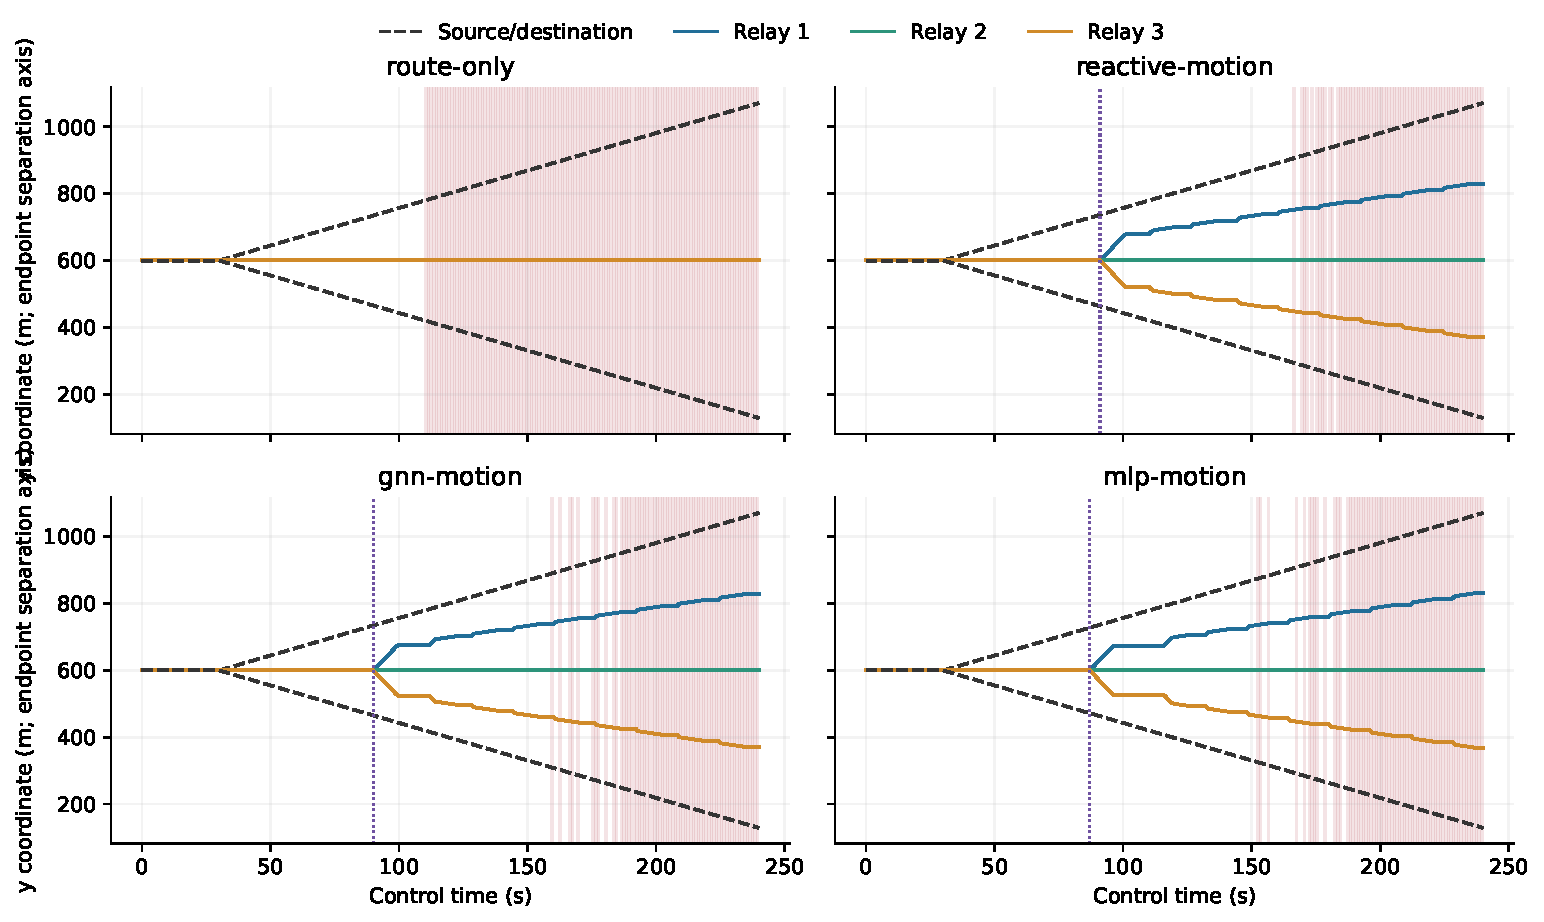
\includegraphics[width=\linewidth]{images/fig_v9_motion_example.pdf}\caption{The n5 gradual episode with the smallest layout seed, shown for all four arms; pale red bands mark probe-graph disconnection and the purple line marks the first commanded motion. The seed was not chosen for a favourable result.}\label{fig:motionexample}\end{figure}

Figure~\ref{fig:motionexample} illustrates the executed actions; the conclusions
are drawn from all scenario blocks. The number of gradual episodes containing
motion is 40/40 for \code{gnn-motion}, 40/40 for \code{mlp-motion}, 40/40 for
\code{reactive-motion} and 0/40 for \code{route-only}.

\subsection{Exploratory analysis: forecasting or smoothing?}\label{sec:posthoc}
The analyses in this section were carried out after the v8 and v9 test results
were available. They were not pre-registered and they do not change the locked
conclusions of either study. They run on fresh seeds and aim to answer
\emph{why} the two studies turned out as they did; their role is explanatory,
not confirmatory.

\subsubsection{A geometric bound on placement control}
Over all node pairs in the 192 v9 test traces, the probability that an edge has
a reception ratio of at least 0.5 was estimated as a function of 3D distance;
that probability falls below 0.5 from about 180~m. Given the actual endpoint
trajectories, an ideal controller that instantaneously equispaces the relays
still incurs a mean of 26.09 disconnected seconds per gradual episode (48.68 for
n5 and 3.51 for n7), assuming independent fading across hops. The reactive
trigger incurs 31.45 seconds and stationary relays 123.43, so the reactive rule
already attains about 94\% of the achievable reduction.

\subsubsection{Forecast error runs opposite to service}
The exploratory study v8x uses 200 fresh episodes over 40 gradual blocks with
the same binary, the same route-pinning rule and the same locked GNN weights;
only the smoothing of current quality changes (Table~\ref{tab:smooth}). All
cells were valid and passed the route integrity checks.
\begin{table}[htbp]
\centering\small
\begin{tabularx}{\linewidth}{@{}Yp{3.6cm}p{2.0cm}@{}}
\toprule
\textbf{Comparison (v8x, gradual)}&\textbf{PDR (points), 95\% CI}&\textbf{Route changes}\\\midrule
\code{gnn-route} $-$ EWMA 0.5&$+0.78$ [0.40, 1.17]&$-7.3$\\
EWMA 0.2 $-$ EWMA 0.5&$+0.78$ [0.42, 1.14]&$-6.0$\\
EWMA 0.1 $-$ EWMA 0.5&$+1.09$ [0.76, 1.43]&$-8.0$\\
Dwell 15 s $-$ EWMA 0.5&$-0.02$ [$-0.31$, 0.27]&$-4.4$\\
\code{gnn-route} $-$ EWMA 0.1&$-0.31$ [$-0.61$, $-0.04$]&$+0.7$\\
\bottomrule
\end{tabularx}
\caption{Exploratory study v8x: paired differences, block bootstrap, balanced between n5 and n7; route-change commands are counted per episode.}\label{tab:smooth}
\end{table}
The GNN gain reproduces on fresh seeds, but a more heavily smoothed EWMA matches
or exceeds it, whereas lengthening the route dwell has no effect. On the same v8
test traces the five-second MSE of EWMA 0.1 (0.00165) is worse than that of EWMA
0.5 (0.00127) and of the GNN (0.00078), even though it delivers the highest PDR,
so forecast accuracy does not explain the PDR benefit. Refitting the GNN and MLP
with five seeds gives MSE values of $0.000778\pm0.000035$ and
$0.001111\pm0.000038$, with the GNN better on all five seeds.

\subsection{Confirmatory study: forecasting versus tuned smoothing}\label{sec:v10}
The three analyses in Section~\ref{sec:posthoc} were performed after the test
results were seen, and the EWMA coefficient 0.1 was itself chosen after v8, so
on their own they cannot settle the question. We therefore pre-registered a
third study (v10, \code{docs/service_v10_protocol.md}, written before the first
cell was run) to test the remaining question directly: once \emph{both} quality
sources are smoothed with the coefficient that is best for each of them, does
the GNN forecast still raise PDR?

Every arm uses the route-pinning rule, the binary, the flags and the locked GNN
weights of v8, with stationary relays. The EWMA family smooths the current
measurement, $q_t=\alpha d_t+(1-\alpha)q_{t-1}$; the GNN family is given the
same knob on the forecast, $q_t=\beta\hat g_t+(1-\beta)q_{t-1}$, where
$\beta=1$ is exactly \code{gnn-route} of v8. The coefficient of each family was
selected on a separate tuning phase of 160 episodes whose seeds are audited
disjoint from every earlier plan including v8x, under a single pre-registered
criterion: the highest n5/n7-balanced mean gradual PDR within the family, ties
broken towards the larger coefficient. Tuning returned 160/160 valid cells and
selected $\alpha^\ast=\beta^\ast=0.1$. Validation returned 60/60 valid cells and
passed its technical gate, and the test returned 144/144 valid cells with route
integrity, forecast traces and relay stationarity verified in every episode.

\begin{table}[htbp]
\centering\small
\begin{tabularx}{\linewidth}{@{}Yp{3.4cm}p{1.9cm}p{2.4cm}@{}}
\toprule
\textbf{Comparison (v10 test)}&\textbf{PDR difference (pp), 95\% CI}&\textbf{n5 / n7}&\textbf{Verdict}\\\midrule
H1: \code{gnn-tuned} $-$ \code{ewma-tuned}&$+0.08$ [$-0.11$, 0.29]&0.18 / $-0.01$&No difference detected\\
H2: \code{ewma-tuned} $-$ \code{lq-route}&$+0.90$ [0.51, 1.35]&1.19 / 0.61&Descriptive only\\
\code{gnn-tuned} $-$ \code{lq-route}&$+0.98$ [0.60, 1.42]&--&Descriptive only\\
\bottomrule
\end{tabularx}
\caption{The v10 test: 40 paired gradual blocks, 10{,}000 block bootstrap resamples, balanced across n5 and n7.}\label{tab:v10test}
\end{table}

\begin{table}[htbp]
\centering\small
\begin{tabularx}{\linewidth}{@{}Yp{2.7cm}p{2.1cm}p{2.0cm}p{1.5cm}@{}}
\toprule
\textbf{Arm}&\textbf{PDR (\%, mean $\pm$ SD)}&\textbf{Route changes (total)}&\textbf{Disconnected (s)}&\textbf{5~s MSE}\\\midrule
\code{lq-route} (EWMA 0.5)&95.08 $\pm$ 2.72&385&31.18&0.00129\\
\code{ewma-tuned} (EWMA 0.1)&95.98 $\pm$ 2.44&83&30.27&0.00166\\
\code{gnn-tuned} (GNN, $\beta=0.1$)&96.07 $\pm$ 2.36&61&30.52&0.00123\\
\bottomrule
\end{tabularx}
\caption{Descriptive statistics for the v10 gradual test; the five-second MSE is computed on the same \code{lq-route} traces, balanced across n5 and n7.}\label{tab:v10means}
\end{table}

The primary endpoint detected no difference (Table~\ref{tab:v10test}): once both
sides are tuned, the GNN leads the EWMA by 0.08 percentage points with a 95\%
confidence interval of $[-0.11, 0.29]$, and it is higher in 22 of 40 gradual
blocks, lower in 16 and tied in 2. Because H1 reached no directional conclusion,
H2 is reported descriptively even though its interval lies above zero; all three
arms deliver the same PDR on the static blocks. Between the two tuned arms the
difference in disconnected time is $+0.25$ seconds, CI $[-0.53, 1.00]$, and the
background-flow PDR difference is $-0.08$ percentage points, CI $[-0.22, 0.06]$.

This confirms the exploratory conclusion through a pre-registered test: the
$+0.66$ percentage point gain of v8 does not require a learned forecaster,
because a tuned one-parameter EWMA reaches the same level ($+0.90$ against the
same untuned EWMA 0.5 baseline). The direction of forecast error also repeats at
confirmatory scale: on the same test traces EWMA 0.1 has the worst five-second
MSE of the three arms (0.00166 against 0.00123 for the smoothed GNN) yet no
worse PDR (Table~\ref{tab:v10means}). Route-change counts fall monotonically
with the amount of smoothing, from 385 to 83 and 61, consistent with the
proposed mechanism: the route-pinning controller behaves better on a less noisy
input, and a learned forecaster smooths as a side effect. The interval
$[-0.11, 0.29]$ still admits a small difference in either direction, so v10 does
not establish equivalence; it shows that whatever gain is attributable to
forecast information as such is smaller than 0.3 percentage points in this
scenario family.

\section{Discussion}
\subsection{Why the routing gain cannot be attributed to forecasting}
Under the route-pinning rule the GNN yields a small but positively bounded gain
over current quality smoothed by an EWMA with coefficient 0.5. That coefficient,
however, was never tuned, and Section~\ref{sec:posthoc} shows that once it is,
an EWMA with coefficient 0.2 matches the GNN exactly while 0.1 exceeds it. The
number of route changes falls under both treatments: 95 commands for the GNN
against 359 for EWMA 0.5. The most plausible mechanism is that the route-pinning
controller behaves better when its input is less noisy, and that a learned
forecaster smooths as a side effect. The v8 gain therefore attaches to
\emph{a more stable quality estimate} rather than to the value of information
about the future.

This reading does not rest on exploratory analysis alone. Study v10
(Section~\ref{sec:v10}) gives both quality sources the same smoothing knob,
selects the coefficient of each family on a separate tuning seed set, and then
tests the remaining difference on fresh test seeds: the result is $+0.08$
percentage points with a confidence interval of $[-0.11, 0.29]$, that is, no
difference detected, while that same one-parameter filter raises PDR by 0.90
percentage points over the untuned baseline of v8. The gain observed in v8
therefore lies in the smoothing parameter rather than in the forecast, and once
that parameter is tuned for both sides the contribution attributable to the
learned model is smaller than 0.3 percentage points.

The strongest evidence for this reading is the direction of forecast error. If
the gain came from forecast information, the more accurate estimator would have
to deliver better service. The opposite holds: on the same test traces the mean
squared error of EWMA 0.1 is 0.00165, worse than EWMA 0.5 (0.00127) and the GNN
(0.00078), yet its PDR is the highest of the three. This is a concrete instance
of a phenomenon already documented in autonomous driving~\cite{closedloop2025},
where rankings under open-loop evaluation do not carry over to closed-loop
evaluation. The GNN-versus-MLP comparison likewise does not isolate the effect
of message passing, because the two models differ in parameter count.

\subsection{Why the placement branch has no headroom left}
The primary endpoint of v9 was not met. The GNN--MLP result has an individually
positive confidence interval but is descriptive only, because the first gate had
already closed. Two reasons compound. The reactive trigger uses a quality
threshold of 0.70 and therefore usually acts before the probe graph partitions
at threshold 0.5; it does not wait for loss of contact before moving, so the
headroom for a five-second forecast was small to begin with. More importantly,
the geometric bound in Section~\ref{sec:posthoc} quantifies that headroom:
ideally and instantaneously equispaced relays still leave 26.09 disconnected
seconds per episode, against 31.45 for the reactive trigger and 123.43 for
stationary relays. The reactive rule already attains about 94\% of the
achievable reduction; what remains lies beyond the coverage range of the relay
chain rather than in the timing of the trigger. In such a situation no
forecaster, however accurate, can improve much.

This is a practically useful conclusion: before investing in a learned policy
for a placement problem, the geometric bound of that problem should be measured.
Other explanations not yet excluded include the velocity domain shift between
the fitting data and the v9 scenarios, and the fact that the model was fitted
only on data with stationary relays.

\subsection{Cost and scope of the comparison with OLSR-ETX}
The largest difference reported in this paper, a PDR 5.75 percentage points
above OLSR-ETX with fast HELLO, is the number that requires the most caution.
Route pinning is centralized control: it has a global view, and in this
simulation telemetry and control commands are not yet transmitted as
channel-contending packets. With the same binary and runtime, study v7 measured
signalling overhead of about 5.55~kB/s for route pinning, comprising 0.29~kB/s
of fallback OLSR, 5.02~kB/s of probes and an estimated 0.25~kB/s of reports to
the controller, against 1.78~kB/s for OLSR-ETX with 0.5~s HELLO and 0.29~kB/s
for plain OLSR. Probes are emitted in every arm, so probe airtime is common,
but the centralized reporting component does not contend for the channel.
The figure of 5.75 percentage points should therefore be read as \emph{an upper
bound for a partially idealized centralized controller}, not as the gain to be
expected once signalling, message loss and control delay are fully simulated.
The cost of route pinning is dominated by the probe rate, a parameter that was
not optimised here.

\subsection{Limitations}
A confidence interval containing zero does not establish equivalence, and no
threshold was changed and no model retrained after the test results were seen.
Identified limitations include a single chain-topology family, a centralized
controller that does not suffer message loss, telemetry traffic that does not
contend for the channel, and the absence of a real UAV trial. In the placement
study the endpoint speed differs from the training data, and relays move
although the fitting data had them stationary. The model was not trained to
compare counterfactual actions; it only triggers a fixed placement rule.
Travelled distance is a geometric cost and was not converted into energy. The
closed-loop studies use a single training seed; refitting with five seeds
preserves the error ordering (the GNN is best on 5/5 seeds), but the closed-loop
PDR of the other seeds has not been measured.

Most important for interpretation: the three analyses in
Section~\ref{sec:posthoc} were performed after the test results were seen, so by
themselves they \emph{explain} the two locked outcomes rather than replacing a
confirmatory test. The EWMA coefficients 0.1 and 0.2 were likewise chosen after
v8 was seen. The most important of those three conclusions was therefore
re-tested by study v10 (Section~\ref{sec:v10}), pre-registered and run on fresh
seeds, which confirms it. The other two remain exploratory: the reversal between
forecast error and service repeats in v10 but was never the locked endpoint of a
study of its own, and the geometric bound is a trace analysis rather than a
hypothesis test. Robustness across training seeds together with a
parameter-matched ablation is pre-registered in
\code{docs/service_v11_protocol.md} and had not been run at the time of writing.
\section{Conclusion}
Two pre-registered studies on chains of five and seven UAVs yield two different
conclusions about one forecaster: a five-second graph regressor improves PDR
when used for route selection against an untuned EWMA, but shows no clear
additional benefit when it only triggers a shared relay placement rule.
Exploratory analyses show that both outcomes have a single explanation: the
routing gain is obtainable with a tuned one-parameter filter, and placement
control is already close to the geometric bound of the problem. The ranking by
forecast error runs opposite to the ranking by service, so in this scenario
family higher forecast accuracy does not buy better service.

A third study, pre-registered once those two outcomes were known, puts that
explanation to a test: when the measurement and the GNN forecast are both tuned
on the same smoothing parameter using a separate tuning set, the remaining PDR
difference is 0.08 percentage points with a confidence interval of
$[-0.11, 0.29]$ and no difference is detected, even though that same parameter
is worth 0.90 percentage points against the untuned baseline. This is a
no-difference result with a narrow interval, not an underpowered test.

The transferable lesson concerns evaluation rather than modelling: a forecaster
should be reported as useful to a network only when it is placed inside the
control loop, compared against a tuned baseline, and measured over paired
scenario blocks. The system and evidence presented here are adequate for a
simulation study of the stated scope and do not establish readiness for flight
deployment.
\section*{Author and data information}
The authors thank M.Sc. Dang Le Bao Chuong for supervising the project.
Nguyen Dinh Tam is the principal investigator and corresponding author.
Code repository: \url{https://github.com/kaing615/UAV-link-quality-routing-support}.
The reproduction package accompanying the manuscript contains the packaged
sources, models, seed plans, results and a SHA-256 manifest; full traces are
archived on the group's server.
\begin{thebibliography}{99}
\bibitem{bekmezci} İ. Bekmezci, O. K. Sahingoz, Ş. Temel.
Flying Ad-Hoc Networks (FANETs): A survey.
\textit{Ad Hoc Networks}, 11(3):1254--1270, 2013.
\bibitem{gupta} L. Gupta, R. Jain, G. Vaszkun.
Survey of important issues in UAV communication networks.
\textit{IEEE Communications Surveys \& Tutorials}, 18(2):1123--1152, 2016.
\bibitem{hayat} S. Hayat, E. Yanmaz, R. Muzaffar.
Survey on unmanned aerial vehicle networks for civil applications:
A communications viewpoint.
\textit{IEEE Communications Surveys \& Tutorials}, 18(4):2624--2661, 2016.
\bibitem{arafat} M. Y. Arafat, S. Moh.
Routing protocols for unmanned aerial vehicle networks: A survey.
\textit{IEEE Access}, 7:99694--99720, 2019.
\bibitem{lakew} D. S. Lakew, U. Sa'ad, N.-N. Dao, W. Na, S. Cho.
Routing in flying ad hoc networks: A comprehensive survey.
\textit{IEEE Communications Surveys \& Tutorials}, 22(2):1071--1120, 2020.
\bibitem{rfc3626} T. Clausen, P. Jacquet.
\textit{Optimized Link State Routing Protocol (OLSR)}. RFC 3626, 2003.
\url{https://www.rfc-editor.org/rfc/rfc3626}.
\bibitem{rfc7181} T. Clausen, C. Dearlove, P. Jacquet, U. Herberg.
\textit{The Optimized Link State Routing Protocol Version 2}. RFC 7181, 2014.
\url{https://www.rfc-editor.org/rfc/rfc7181}.
\bibitem{decouto} D. S. J. De Couto, D. Aguayo, J. Bicket, R. Morris.
A high-throughput path metric for multi-hop wireless routing.
\textit{Proc. ACM MobiCom}, 2003.
\bibitem{draves} R. Draves, J. Padhye, B. Zill.
Routing in multi-radio, multi-hop wireless mesh networks.
\textit{Proc. ACM MobiCom}, pp. 114--128, 2004.
\bibitem{olsrd} olsr.org. \textit{olsrd: an ad hoc wireless mesh routing
daemon} (link quality extension). \url{https://github.com/OLSR/olsrd}.
\bibitem{baccour} N. Baccour, A. Koubâa, L. Mottola, M. A. Zúñiga, H. Youssef,
C. A. Boano, M. Alves. Radio link quality estimation in wireless sensor
networks: A survey. \textit{ACM Transactions on Sensor Networks}, 8(4), 2012.
\bibitem{cerar} G. Cerar, H. Yetgin, M. Mohorčič, C. Fortuna.
Machine learning for wireless link quality estimation: A survey.
\textit{IEEE Communications Surveys \& Tutorials}, 23(2), 2021.
\url{https://arxiv.org/abs/1812.08856}.
\bibitem{shi2024} J. Shi et al.
Limitations and benefits of link quality prediction in stochastic wireless
multihop networks. \textit{International Journal of Distributed Sensor
Networks}, 2024. \url{https://doi.org/10.1155/2024/9546316}.
\bibitem{kipf} T. N. Kipf, M. Welling.
Semi-supervised classification with graph convolutional networks.
\textit{ICLR}, 2017.
\bibitem{graphsage} W. L. Hamilton, R. Ying, J. Leskovec.
Inductive representation learning on large graphs.
\textit{NeurIPS}, 2017. \url{https://arxiv.org/abs/1706.02216}.
\bibitem{gat} P. Veličković, G. Cucurull, A. Casanova, A. Romero, P. Liò,
Y. Bengio. Graph attention networks. \textit{ICLR}, 2018.
\bibitem{xgboost} T. Chen, C. Guestrin.
XGBoost: A scalable tree boosting system.
\textit{Proc. ACM KDD}, pp. 785--794, 2016.
\bibitem{routenet} K. Rusek, J. Suárez-Varela, P. Almasan, P. Barlet-Ros,
A. Cabellos-Aparicio. RouteNet: Leveraging graph neural networks for network
modeling and optimization in SDN.
\textit{IEEE Journal on Selected Areas in Communications}, 38(10):2260--2270, 2020.
\bibitem{bai2025} Y. Bai et al.
Link prediction of UAV networks based on dynamic graph neural network.
\textit{IET Communications}, 2025. \url{https://doi.org/10.1049/cmu2.70092}.
\bibitem{gnnppor} Y. Song et al.
GNNPPOR: A proximal policy optimization multi-factor joint routing approach
based on graph neural networks in FANETs.
\textit{IEEE Networking Letters}, 2025.
\bibitem{drones2026} Graph neural network-enabled intelligence for unmanned
aerial vehicle systems: A comprehensive review.
\textit{Drones}, 2026. \url{https://doi.org/10.3390/drones10070548}.
\bibitem{qmr} J. Liu, Q. Wang, C. He, K. Jaffrès-Runser, Y. Xu, Z. Li, Y. Xu.
QMR: Q-learning based multi-objective optimization routing protocol for flying
ad hoc networks. \textit{Computer Communications}, 150:304--316, 2020.
\bibitem{rosati2013} S. Rosati, K. Kruzelecki, L. Traynard, B. Rimoldi.
\textit{Speed-Aware Routing for UAV Ad-Hoc Networks}.
arXiv:1307.6350, 2013. \url{https://arxiv.org/abs/1307.6350}.
\bibitem{liu2025} J. Liu, P. Gong, H. Yang, S. Li, X. Gao.
Cross-layer optimized OLSR protocol for FANETs in interference-intensive
environments. \textit{Drones}, 9(11):778, 2025.
\url{https://doi.org/10.3390/drones9110778}.
\bibitem{zeng2016} Y. Zeng, R. Zhang, T. J. Lim.
Throughput maximization for UAV-enabled mobile relaying systems.
\textit{IEEE Transactions on Communications}, 64(12):4983--4996, 2016.
\bibitem{abir} M. A. B. S. Abir, M. Z. Chowdhury, Y. M. Jang.
Software-defined UAV networks for 6G systems: Requirements, opportunities,
emerging techniques, challenges, and research directions.
\textit{IEEE Open Journal of the Communications Society}, 4:2487--2547, 2023.
\bibitem{closedloop2025} Closing the loop: Motion prediction models beyond
open-loop benchmarks. arXiv:2505.05638, 2025.
\url{https://arxiv.org/abs/2505.05638}.
\bibitem{lin2018} J. Lin.
The neural hype and comparisons against weak baselines.
\textit{ACM SIGIR Forum}, 52(2):40--51, 2018.
\url{https://doi.org/10.1145/3308774.3308781}.
\bibitem{mcgreivy2024} N. McGreivy, A. Hakim.
Weak baselines and reporting biases lead to overoptimism in machine learning
for fluid-related partial differential equations.
arXiv:2407.07218, 2024. \url{https://arxiv.org/abs/2407.07218}.
\bibitem{nosek} B. A. Nosek, C. R. Ebersole, A. C. DeHaven, D. T. Mellor.
The preregistration revolution.
\textit{Proceedings of the National Academy of Sciences}, 115(11):2600--2606, 2018.
\bibitem{efron1993} B. Efron, R. J. Tibshirani.
\textit{An Introduction to the Bootstrap}. Chapman \& Hall, 1993.
\bibitem{ns3} ns-3 Network Simulator, version 3.45. \url{https://www.nsnam.org/}.
\end{thebibliography}
\end{document}
